\documentclass[UTF8,fontset=windows,11pt,a4paper]{ctexart}
\usepackage[margin=2.05cm]{geometry}
\usepackage{amsmath,amssymb,booktabs,tabularx,array,multirow,longtable}
\usepackage{graphicx,xcolor,enumitem,fancyhdr,hyperref,xurl,float,caption}
\graphicspath{{../figures/}}

\definecolor{ok}{RGB}{25,120,70}
\definecolor{blue}{RGB}{35,75,130}
\definecolor{shade}{RGB}{245,247,250}
\hypersetup{
  colorlinks=true,
  linkcolor=blue,
  urlcolor=blue,
  pdfauthor={FG-MEE numerical validation workbench},
  pdftitle={FG-MEE 板壳最新可行数值结果报告}
}
\pagestyle{fancy}
\fancyhf{}
\lhead{FG-MEE 板壳最新可行数值结果}
\rhead{2026-07-19 修订}
\cfoot{\thepage}
\setlength{\headheight}{15pt}
\setlength{\parindent}{2em}
\setlength{\parskip}{0.28em}
\renewcommand{\arraystretch}{1.16}
\captionsetup{font=small,labelfont=bf}
\newcommand{\pass}{\textcolor{ok}{\textbf{通过}}}
\newcommand{\tierA}{\textcolor{ok}{\textbf{A 级}}}
\newcommand{\tierB}{\textcolor{blue}{\textbf{B 级}}}
\newcolumntype{Y}{>{\raggedright\arraybackslash}X}
% Auto-generated by tools/analyze_curvature_fg_full_validation.py
\newcommand{\MaxCurvatureChange}{0.00787753}
\newcommand{\CurvatureGateConclusion}{四个半径中有 4/4 个半径的六类中心位移全部通过 1\% 门槛，其中 4/4 个也通过 0.5\% 优先门槛；全表最大变化为 0.00787753\%。}
\newcommand{\FullRadiusStatus}{\pass}
\newcommand{\InteractionConclusion}{12 个半径--载荷交互中有 12 个高于三倍离散界；绝对值最大者位于 $R=1.0$ m 的电致工况，为 1.5421 个百分点。同一半径电致与磁致交互的最大差仅为 1.602e-08 个百分点，符合线性结构响应下的归一化一致性；机械工况有 4/4 个半径达到已分辨标准。}
\newcommand{\RadiusSummaryRows}{%
1.0 & 1.0 & 0.0079 & 0.0042 & 通过 \\
0.4 & 2.5 & 0.0059 & 0.0025 & 通过 \\
0.3 & 3.3 & 0.0053 & 0.0027 & 通过 \\
0.2 & 5.0 & 0.0046 & 0.0026 & 通过 \\
}
\newcommand{\InteractionRows}{%
1.0 & 机械 & -0.0999 & 0.0079 & 12.7 & 已分辨 \\
1.0 & 电致 & 1.5421 & 0.0032 & 479.6 & 已分辨 \\
1.0 & 磁致 & 1.5421 & 0.0032 & 479.6 & 已分辨 \\
0.4 & 机械 & -0.0473 & 0.0059 & 8.1 & 已分辨 \\
0.4 & 电致 & 1.4942 & 0.0015 & 977.1 & 已分辨 \\
0.4 & 磁致 & 1.4942 & 0.0015 & 977.1 & 已分辨 \\
0.3 & 机械 & -0.0362 & 0.0053 & 6.8 & 已分辨 \\
0.3 & 电致 & 1.4285 & 0.0020 & 706.4 & 已分辨 \\
0.3 & 磁致 & 1.4285 & 0.0020 & 706.4 & 已分辨 \\
0.2 & 机械 & -0.0266 & 0.0046 & 5.7 & 已分辨 \\
0.2 & 电致 & 1.3568 & 0.0023 & 596.9 & 已分辨 \\
0.2 & 磁致 & 1.3568 & 0.0023 & 596.9 & 已分辨 \\
}

\setcounter{tocdepth}{2}

\title{\textbf{FG-MEE 板壳最新可行数值结果报告}\\[0.35em]
\large MATLAB--COMSOL 同构验证、全半径曲率响应与位移反问题审计}
\author{FG-MEE 数值验证工作台}
\date{2026年7月19日修订}

\begin{document}
\maketitle

\begin{abstract}
本文汇总截至 2026 年 7 月 19 日已经完成复算的 FG-MEE 板壳数值实验结果。首先，在 $300\,\mathrm{mm}\times300\,\mathrm{mm}\times6\,\mathrm{mm}$ 悬臂平板上建立 MATLAB H20 与 COMSOL 二次巧凑三维实体同构模型；10/15/20 三档面内网格、两类外应力载荷的中心位移最大相对差为 $1.7690\times10^{-4}\%$，自由端中点最大相对差为 $1.2127\times10^{-4}\%$。平板压力、电致和磁致结果另与 Zhang 等（钱沈云为合著者）的已发表表格核对，同工况差异为 $0.010\%$--$0.92\%$。其次，对 $R=1.0,0.4,0.3,0.2$ m 四个曲率半径、U/X 两种厚度分布及压力、电致、磁致三类载荷完成 20/30 网格复算；24 个正式工况的最大网格变化为 $0.00787753\%$。代表性的 $R=0.4$ m 独立 COMSOL 三维曲壳在 15 到 20 网格间变化为 $0.9651\%$，其与 MATLAB LRT5 的 $8.0830\%$ 差异作为非同构模型形式敏感性报告。最后，本次将“达到目标位移所需的外加载势”和“给定位移后的局部感生势后处理”严格分开：0.5 mm 目标下，MATLAB/COMSOL 加载反算分别为 $2870.424/2591.274$ V 和 $572.784/524.202$ A；两条非同构链分别用自身灵敏度完成自洽回代，COMSOL 数值是独立备选估计，不是对 MATLAB 载荷的同构验证。把 MATLAB 载荷原样施加到 COMSOL 后实际得到 0.553863 mm 和 0.546340 mm，分别比目标高 10.7726\% 和 9.2679\%，从而直接量化了跨模型差异。原 $78.4803$ V 和 $0.0309000$ A 是在无外加热源但保留热--机互易温度响应时得到的层均势自由度极差，COMSOL 侧也只求三维力学场后采用同一代数本构，不能作为独立传感 PDE 或外加载势证据。钱沈云相关旧程序的较大感生势已定位到热释电/热释磁矩阵在十层自由度上的重复装配，因而同源复跑不能替代独立正确性验证。

\noindent\textbf{关键词：}功能梯度磁电弹；MATLAB；COMSOL；同构验证；曲壳；加载反算；感生势
\end{abstract}

\begin{center}
\fcolorbox{blue}{shade}{
\begin{minipage}{0.93\textwidth}
\textbf{核心结论。}
在严格统一单元族、三维运动学、材料、边界、载荷与探针后，MATLAB--COMSOL 的最大差异低于 $0.00018\%$；平板三类载荷与前人公开表格的差异为 $0.010\%$--$0.92\%$。四个正文半径的 24 个曲壳工况全部通过 0.5\% 网格门槛。位移反问题已经拆成两条链：MATLAB 与 COMSOL 的外加载势反算分别完成各自正向模型的自洽回代，不能把 COMSOL 自回代写成 MATLAB 值的独立证明；MATLAB 的 0.5 mm 反算载荷交叉施加到 COMSOL 后超出目标 9.27\%--10.77\%。局部感生势仍只是“力学场 + 同一本构后处理”，必须降级为探索性结果，不能再把 $78.4803$ V、$0.0309000$ A 称为产生 0.5 mm 位移所需的加载势，也不能把相同的 3.4654\% 当成两个独立电磁验证样本。
\end{minipage}}
\end{center}

\newpage
\begingroup
\scriptsize
\setlength{\parskip}{0pt}
\tableofcontents
\endgroup
\newpage

\section{研究问题、范围与证据口径}

\subsection{问题来源与报告目标}

本研究需要回答的核心问题不是“两个软件能否给出大致相同的图形”，而是偏差来自哪里、每一类偏差能够支持什么结论。若 MATLAB 与 COMSOL 在同一材料、同一边界、同一载荷和同一输出位置下仍相差 2\% 左右，单纯把差异归为“正常软件误差”并不充分，因为求解器差异、网格差异、模型降维差异和后处理定义差异可能同时存在。为避免这些因素互相遮蔽，本文把验证链拆成平板外部基准、三维实体同构闭合、曲壳网格复算、独立三维曲壳、外加载势反算与感生势审计六个模块，并分别给出其证据边界。

本报告只纳入截至 2026 年 7 月 19 日可重复运行的最终数据，不把调试失败值、旧装配值或中间截图作为正文结果。本文把 MATLAB/COMSOL 求解、网格复算、参数扫描与跨软件对照统称为\textbf{数值实验}，这些工作已经实际完成。这里的“实验”指在受控参数下反复运行数值模型并比较输出，不等同于实体样件试验。尚未开展的是样件制备以及由位移计、电压表或磁测量装置参与的台架测量，因此算法一致性、离散收敛和参数规律可以由当前数值实验支撑，而真实器件的输出能力仍不能由本文直接宣称。

\subsection{待回答的五个数值问题}

本文围绕表~\ref{tab:research_questions}中的五个问题组织结果。前两个问题用于判断平板正向模型是否可信；第三个问题建立小论文的曲率--材料分布主结果；第四个问题检验降维板壳相对三维实体的模型敏感性；第五个问题分别评估外加载势反算是否完成正向回代、感生势链是否已经达到可报告状态。这样组织后，“误差小”不再是单一结论，而是必须明确误差分母、模型层级与比较对象的定量判断。

\begin{table}[H]
\centering
\caption{研究问题及对应的判定证据}
\label{tab:research_questions}
\scriptsize
\begin{tabularx}{\textwidth}{p{0.09\textwidth}Xp{0.30\textwidth}}
\toprule
编号 & 研究问题 & 主要证据 \\
\midrule
Q1 & 当前平板压力、电致和磁致位移是否处于前人同工况结果的合理误差量级？ & 已发表模型与 COMSOL 表格对照 \\
Q2 & 在运动学、网格、载荷与探针完全统一后，MATLAB 与 COMSOL 是否仍存在百分数级差异？ & H20--二次实体双探针同构比较 \\
Q3 & 曲率和 U/X 厚度分布怎样改变三类载荷的中心位移，规律是否高于离散误差？ & 四半径、两分布、三载荷的 20/30 网格复算 \\
Q4 & 降维 LRT5 曲壳与独立三维曲壳之间存在多大模型形式差异？ & $R=0.4$ m 独立 COMSOL 曲壳网格序列 \\
Q5 & 两条非同构致动链能否分别自洽回代、交叉施加载荷后相差多少；感生势是否已有独立场方程证据？ & 正向灵敏度反算、COMSOL 自回代与 MATLAB 载荷交叉施加、感生势证据审计 \\
\bottomrule
\end{tabularx}
\end{table}

\subsection{证据等级与结论强度}

数值证据按模型是否同构分级。A 级要求两个求解器共享几何、材料、边界、载荷实现、单元运动学与输出位置，因而其差异可以解释为实现层面的跨求解器差异。B 级允许自由度、运动学或后处理链不同，只用于检验符号、量级、趋势及模型敏感性。外部基准则用于判断当前结果是否落在已发表同工况的数值范围内，但不会因为引用了公开结果就自动成为同构证据。

\begin{table}[H]
\centering
\caption{本文纳入的结果及其证据边界}
\small
\begin{tabularx}{\textwidth}{p{0.24\textwidth}Xp{0.16\textwidth}}
\toprule
结果模块 & 可支持的结论 & 等级 \\
\midrule
MATLAB H20--COMSOL 二次实体 & 外应力机械核的跨软件实现一致性 & \tierA \\
平板三类载荷前人表格 & 同几何、同载荷下的外部数值基准一致性 & \textbf{外部基准} \\
四半径 20/30 网格复算 & MATLAB 曲壳响应的离散收敛与参数趋势 & \tierA \\
$R=0.4$ m 独立 COMSOL 曲壳 & 三维曲壳自身收敛及 LRT5 模型形式敏感性 & \tierB \\
目标位移--外加载势反算 & 两条非同构链的自身回代及 MATLAB 载荷向 COMSOL 的交叉施加 & \tierB \\
机械变形--开路感生势 & 当前层均势极差定义及局部本构条件性；尚无独立场 PDE & \textbf{探索性} \\
\bottomrule
\end{tabularx}
\end{table}

表中的六类证据构成由“已发表量级”到“同构实现”、再到“非同构模型敏感性和未闭合探索项”的递进结构。A 级同构闭合回答代码与软件实现是否一致；网格复算回答离散结果是否稳定；B 级比较回答模型形式改变后结果会移动多少；探索性结果只用于暴露数据定义和待验证假设。四者不能用一个统一百分比替代，也不能把非同构的 8\%--10\% 加载差解释为 MATLAB 或 COMSOL 的求解错误，更不能把感生势共享后处理差写成独立 PDE 验证。本文后续所有结论均沿用这一口径。

\section{理论模型与评价指标}

\subsection{几何、材料分布与载荷}

主体结构的轴向长度、弧长和厚度分别为 300 mm、300 mm 和 6 mm，厚度划分为 10 个物理层。曲壳的周向起始端 $s=R\theta=0$ 固支，其余三个结构边自由；若将局部周向坐标记为 $x$，该边界即通常所写的 $x=0$ 固支。曲壳半径取 $R=1.0,0.4,0.3,0.2$ m，对应曲率 $1/R=1.0,2.5,3.33,5.0\ \mathrm{m}^{-1}$。材料为 BaTiO$_3$/CoFe$_2$O$_4$ 混合体系，当前比较使用两种厚度分布：
\[
V_{\mathrm{BTO}}^{U}(z)=0.6,
\qquad
V_{\mathrm{BTO}}^{X}(z)=0.6\frac{|z|}{h/2},
\qquad -\frac{h}{2}\le z\le\frac{h}{2}.
\]
U 表示厚度均匀分布，X 表示上下表面富 BaTiO$_3$、中面富 CoFe$_2$O$_4$ 的对称分布。三类正向载荷分别为 15 kPa 横向压力、每个 0.6 mm 外侧活动层内的 300 V 电势差和 200 A 磁标势差；其中 200 A 是磁标势之差，不表示 200 A 电流。主要输出为几何中心的法向位移 $w_c$。

图~\ref{fig:curved_geometry_loads}以统一物理尺度给出四个有限半径的圆柱壳几何、CFFF 边界、压力方向及位置标记。半径减小时，弧长保持 300 mm，故圆心角由 $17.19^{\circ}$ 增至 $85.94^{\circ}$。图~\ref{fig:material_boundary_loads}进一步画出十层 U/X 材料分布以及三类载荷的实际作用方式。直接场复算中，上下两侧外表面均施加 $\phi=300$ V、$\psi=200$ A，相邻内界面取 $\phi=0$ V、$\psi=0$ A，因此上下活动层沿全局 $z$ 方向的势梯度与场强符号相反。

\begin{figure}[H]
\centering
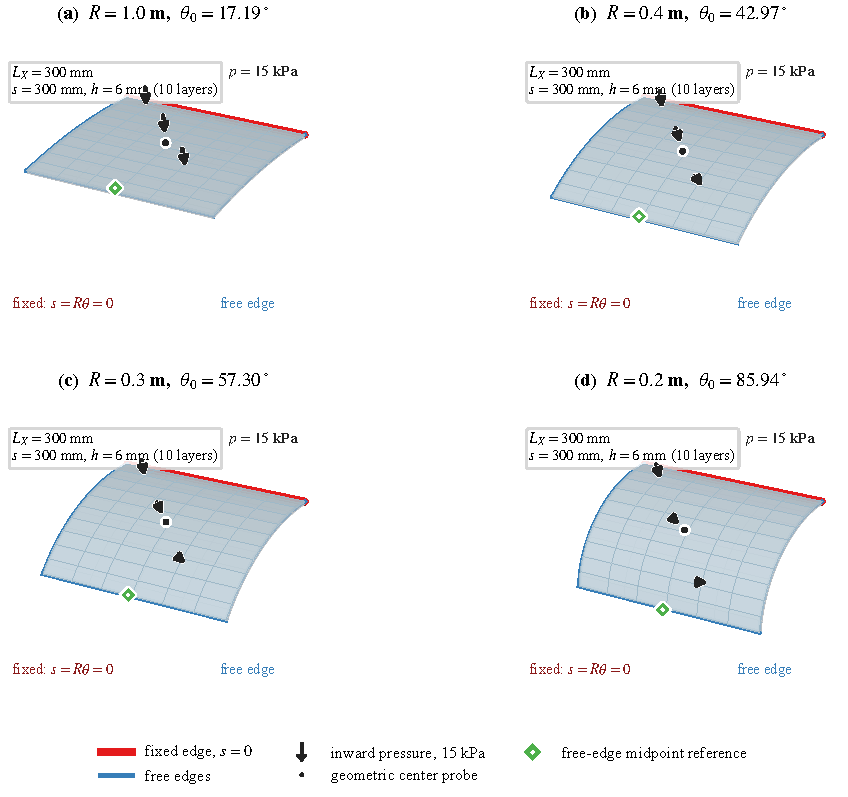
\includegraphics[width=0.98\textwidth]{Fig_00_curved_shell_geometry_loads.pdf}
\caption{四种曲率半径的圆柱壳几何、边界、压力与位置标记。红色边为周向起始固支端 $s=R\theta=0$，蓝色为自由边，黑色箭头表示 15 kPa 外表面法向压力；黑点为曲壳正式输出采用的几何中心探针，绿色菱形仅标示自由边中点几何参考位置，用于对应后文平板同构双探针说明。标记为便于观察而沿外法向略作显示偏移，不改变实际坐标。四幅图采用相同坐标尺度，厚度按实际 6 mm 建模。}
\label{fig:curved_geometry_loads}
\end{figure}

\begin{figure}[H]
\centering
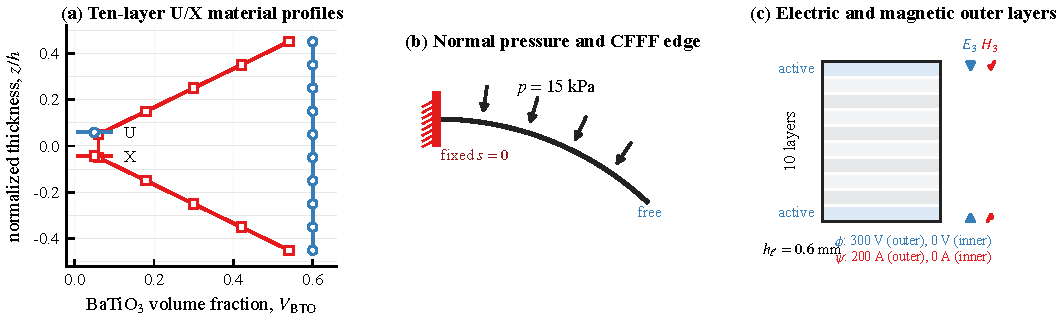
\includegraphics[width=0.98\textwidth]{Fig_00_material_boundary_loads.pdf}
\caption{十层材料、边界与载荷方式示意。（a）U/X 两种 BaTiO$_3$ 体积分数分布；（b）CFFF 固支边与 15 kPa 法向压力，箭头按圆柱截面的真实径向绘制；（c）上下两个 0.6 mm 外侧活动层的电势与磁标势边界，蓝色实线箭头和红色虚线箭头分别表示 $E_3$、$H_3$ 方向，不表示机械力。}
\label{fig:material_boundary_loads}
\end{figure}

结构长厚比为 $L/h=50$，而有限半径工况的无量纲厚度曲率 $h/R$ 为 0.006--0.030。由于弧长固定为 0.3 m，半径减小时圆心角显著增大；$R=0.2$ m 已对应约 $85.94^{\circ}$ 的圆柱扇段。表~\ref{tab:dimensionless_curvature}给出这些量。该组参数既覆盖接近平板的弱曲率状态，也包含几何弯曲较强的状态，因此不能预设响应必然随 $1/R$ 线性变化。

\begin{table}[H]
\centering
\caption{有限半径工况的几何无量纲参数}
\label{tab:dimensionless_curvature}
\begin{tabular}{rrrr}
\toprule
$R$/m & $1/R$/m$^{-1}$ & 圆心角/(deg) & $h/R$ \\
\midrule
1.0 & 1.0000 & 17.1887 & 0.006 \\
0.4 & 2.5000 & 42.9718 & 0.015 \\
0.3 & 3.3333 & 57.2958 & 0.020 \\
0.2 & 5.0000 & 85.9437 & 0.030 \\
\bottomrule
\end{tabular}
\end{table}

\subsection{MEE 耦合本构与逐层材料混合}

在线性、小变形假设下，磁电弹材料采用应力--电位移--磁感应强度形式的耦合本构：
\[
\begin{aligned}
\boldsymbol\sigma
  &=\mathbf C\boldsymbol\varepsilon-\mathbf e^{\mathsf T}\mathbf E
    -\mathbf q^{\mathsf T}\mathbf H-\boldsymbol\lambda\Delta T,\\
\mathbf D
  &=\mathbf e\boldsymbol\varepsilon+\boldsymbol\chi\mathbf E
    +\boldsymbol\kappa\mathbf H+\mathbf p_E\Delta T,\\
\mathbf B
  &=\mathbf q\boldsymbol\varepsilon+\boldsymbol\kappa^{\mathsf T}\mathbf E
    +\boldsymbol\gamma\mathbf H+\mathbf p_M\Delta T.
\end{aligned}
\]
其中，$\boldsymbol\sigma$、$\boldsymbol\varepsilon$、$\mathbf E$、$\mathbf H$、$\mathbf D$ 和 $\mathbf B$ 分别为应力、应变、电场、磁场、电位移和磁感应强度；$\mathbf C$、$\mathbf e$、$\mathbf q$、$\boldsymbol\chi$、$\boldsymbol\kappa$ 和 $\boldsymbol\gamma$ 依次表示弹性、压电、压磁、介电、磁电和磁导系数。本文正文正向载荷工况取 $\Delta T=0$，保留温度项用于说明完整本构结构。后文对钱沈云相关旧反推程序的审计会单独讨论其非零温度响应；零温工况与含热释项工况不得混为同一组结果。

厚度方向划分为 10 个物理层。对任一层 $k$，全部材料参数按 BaTiO$_3$ 与 CoFe$_2$O$_4$ 的体积分数作同一线性混合：
\[
\mathbf P_k
=V_{\mathrm{BTO}}(z_k)\mathbf P_{\mathrm{BTO}}
+\left[1-V_{\mathrm{BTO}}(z_k)\right]\mathbf P_{\mathrm{CFO}},
\]
其中 $\mathbf P$ 统一代表上述弹性、压电、压磁、介电、磁电和磁导参数。U/X 比较中几何、边界、载荷和层数保持不变，但必须注意两种分布的厚度平均体积分数并不相同：U 分布的 $\overline V_{\mathrm{BTO}}=0.6$，X 分布对厚度积分后的 $\overline V_{\mathrm{BTO}}=0.3$。因此，原始 U/X 位移差异同时包含\textbf{平均组分变化}和\textbf{厚度重分布}，不能被表述为保持总组分不变的纯梯度效应。后文使用各自平板结果归一化，是为了尽可能剥离这一基线差异，重点识别曲率对两种分布相对响应的调制。

十层物理离散采用层中点体积分数。对称 X 分布使上下半层参数成对相同，不引入人为的膜--弯耦合不对称；但材料刚度与压电、压磁系数仍随 $|z|$ 变化，因而弯曲应变在厚度方向的加权方式与 U 分布不同。该差异是解释压力、电致和磁致结果分化的关键，而不是简单比较某一个材料常数即可得到的结论。

\subsection{LRT5 板壳离散与正反向载荷链}

MATLAB 曲壳模型采用五参数一阶板壳运动学。局部坐标下的位移写为
\[
u(x,y,z)=u_0(x,y)+z\beta_x(x,y),\qquad
v(x,y,z)=v_0(x,y)+z\beta_y(x,y),\qquad
w(x,y,z)=w_0(x,y),
\]
即中面三个位移与两个转角共同描述板壳变形。逐层积分后的单元机械刚度可概括为
\[
\mathbf K_{uu}^{e}
=\int_{\Omega_e}\sum_{k=1}^{10}
  \int_{z_k^-}^{z_k^+}
  \mathbf B_u^{\mathsf T}\mathbf C_k\mathbf B_u
  \,\mathrm dz\,\mathrm d\Omega .
\]
在规定外载、电势或磁标势时，静力正向方程写为
\[
\mathbf K_{uu}\mathbf Q_d
=\mathbf F_{\mathrm{mech}}
-\mathbf K_{u\phi}\boldsymbol\Phi_a
-\mathbf K_{u\psi}\boldsymbol\Psi_a,
\]
分别给出压力、电致和磁致位移。由正向模型得到固定载荷形态下的中心位移灵敏度
\[
S_\phi=\frac{w_c}{\Phi_a},\qquad
S_\psi=\frac{w_c}{\Psi_a},
\]
后，达到目标绝对位移 $|w^*|$ 所需的外加载势为
\[
|\Phi_{\mathrm{req}}|=\frac{|w^*|}{|S_\phi|},\qquad
|\Psi_{\mathrm{req}}|=\frac{|w^*|}{|S_\psi|}.
\]
这是后文所称的\textbf{加载反算}。它只在当前线性、小变形和载荷空间分布不变的条件下成立，必须再把反算载荷代回正向场模型检查目标位移。

另一类问题是机械变形后的\textbf{感生势反算}。在规定位移 $\mathbf Q_d$、温度差 $\Delta\mathbf T$ 和电/磁参考势后，完整离散方程为
\[
\begin{bmatrix}
\mathbf K_{\phi\phi} & \mathbf K_{\phi\psi}\\
\mathbf K_{\psi\phi} & \mathbf K_{\psi\psi}
\end{bmatrix}
\begin{bmatrix}\boldsymbol\Phi_s\\\boldsymbol\Psi_s\end{bmatrix}
=-
\begin{bmatrix}
\mathbf K_{\phi u}\mathbf Q_d+\mathbf K_{\phi T}\Delta\mathbf T+\mathbf G\\
\mathbf K_{\psi u}\mathbf Q_d+\mathbf K_{\psi T}\Delta\mathbf T+\mathbf M
\end{bmatrix}.
\]
其中 $\mathbf G$、$\mathbf M$ 表示电荷与磁通边界源项。只有明确浮置电极、零净自由电荷、磁势规范条件、温度边界及端子输出定义后，$\boldsymbol\Phi_s$、$\boldsymbol\Psi_s$ 才具有可比的物理含义。加载反算与感生势反算的未知量和边界条件不同；后续不再用同一“位移反推势”名称混称二者。

\subsection{三维实体同构核与比较条件}

为把“软件差异”从“板壳理论差异”中分离，本文另建三维实体机械核。MATLAB 使用 20 节点巧凑六面体 H20 单元和 $3\times3\times3$ 高斯全积分；COMSOL 采用二次巧凑三维实体。两者不调用 LRT5 转角自由度，而是在相同三维坐标、相同厚度分层与相同外应力上直接求位移。只有这一组模型满足单元运动学层面的同构条件。

同构不是“输入文件看起来相似”，而是至少同时满足六项约束：几何节点位置一致、材料参数一致、固定自由度一致、载荷的作用面和符号一致、单元插值阶次一致、探针坐标与位移分量一致。任一约束未统一时，所得差异都可能包含模型或后处理因素。表~\ref{tab:isomorphic_conditions}把本文实际采用的对齐项明确列出。

\begin{table}[H]
\centering
\caption{MATLAB H20--COMSOL 二次实体同构条件}
\label{tab:isomorphic_conditions}
\small
\begin{tabularx}{\textwidth}{p{0.19\textwidth}XX}
\toprule
对齐项 & MATLAB & COMSOL \\
\midrule
几何与分层 & $300\times300\times6$ mm，10 个厚度单元 & 同尺寸，每物理层 1 个厚度单元 \\
单元族 & 20 节点巧凑六面体，全积分 & 二次巧凑三维实体 \\
材料 & $E=1.206\times10^{11}$ Pa，$\nu=0.3398$ & 同一 $E$、$\nu$ \\
边界 & $x=0$ 端面三向位移固定 & 同一端面固定 \\
载荷 & 最外两层等值反向面内外应力 & 同一层、同一应力符号与数值 \\
输出 & 几何中心与自由端中点的 $w$ & 同坐标、同分量点探针 \\
\bottomrule
\end{tabularx}
\end{table}

\subsection{误差、网格变化与交互量}

跨软件相对误差和相邻网格变化统一定义为
\[
\varepsilon_{AB}=100\frac{|w_A-w_B|}{|w_A|},
\qquad
\eta_{20\rightarrow30}=100\frac{|w_{30}-w_{20}|}{|w_{30}|}.
\]
同构跨软件验收门槛为 $\varepsilon_{AB}\le0.1\%$；曲率扫描的网格变化优先门槛为 $\eta_{20\rightarrow30}\le0.5\%$。为识别曲率与材料分布的非加性交互，先以同模式的 30$\times$30 平板结果归一化，再定义
\[
I_R=100\left[
\frac{|w_X(R)|}{|w_X(\infty)|}
-\frac{|w_U(R)|}{|w_U(\infty)|}
\right]\quad\text{(百分点)}.
\]
当 $|I_R|$ 超过同半径、同载荷 U/X 最大网格变化的三倍时，记为“已分辨”。

上述指标分别回答不同问题。$\varepsilon_{AB}$ 是同一离散模型在两个求解器之间的实现一致性；$\eta_{20\rightarrow30}$ 是单一求解器随离散细化的稳定性；$I_R$ 则比较曲率使 U/X 归一化响应产生的相对分离。特别是，$I_R$ 的单位为百分点，不是位移的相对误差。本文还同时报告绝对差值，因为当位移量级较小时，仅看相对百分比容易放大或掩盖实际数值尺度。

门槛用于组织证据，而不是宣称普遍行业标准。0.1\% 的同构门槛对应本研究对机械核闭合的严格要求；0.5\% 的曲率网格门槛用于保证参数趋势不由 20/30 离散差主导；独立三维曲壳采用 1\% 门槛，是因为该模型计算规模更高且目的在于模型形式敏感性。任何通过门槛的结果仍需结合比较对象和绝对差解释。

\section{平板基准与前人结果对照}

\subsection{比较对象与测点定义}

旧报告中仍可直接支撑当前正文的外部证据，是相同平板几何、边界和载荷下的已发表表格数据。本文将当前 MATLAB 结果与 Zhang 等的全耦合板模型及其 COMSOL 结果逐项对照\footnote{S.-Q. Zhang, S.-Y. Qian, S. Liu, C.-Y. Ling and S.-Y. Ma, ``Fully coupled modeling for static and dynamic analysis of thermo-magneto-electro-elastic plates,'' \emph{International Journal of Mechanics and Materials in Design}, vol.~22, article~17, 2026, \href{https://doi.org/10.1007/s10999-025-09834-9}{doi:10.1007/s10999-025-09834-9}.}。压力工况比较自由端中点，电致和磁致工况比较几何中心，三类测点定义不混用。

压力结果采用自由端中点，是因为悬臂板该处的弯曲位移比中心更能反映整体柔度；电致和磁致结果沿用文献表格的中心点定义。本文保留位移正负号用于检查载荷方向，但误差计算采用绝对差与参考值绝对值，避免相反符号被错误地抵消。由于这组对照的模型实现与当前代码并非自由度级同构，其作用是建立外部量级锚点，而不是替代下一节的独立同构验证。

\begin{table}[H]
\centering
\caption{平板三类载荷与已发表表格结果对照}
\label{tab:published_flat_benchmark}
\small
\begin{tabular}{@{}lrrrr@{}}
\toprule
工况（测点） & 本文/mm & 文献模型/mm & 文献 COMSOL/mm & 差异（模型/COMSOL） \\
\midrule
15 kPa，自由端中点 & $-5.99822273$ & $-5.9976$ & $-5.9525$ & $0.010\%/0.768\%$ \\
300 V，中心点 & $-0.05225709$ & $-0.0523$ & $-0.0523$ & $0.08\%/0.08\%$ \\
200 A，中心点 & $0.17458575$ & $0.175$ & $0.173$ & $0.24\%/0.92\%$ \\
\bottomrule
\end{tabular}
\end{table}

\subsection{相对差与绝对差的联合解释}

三类载荷的同工况差异为 $0.010\%$--$0.92\%$，均低于 1\% 量级，可作为当前平板正向计算的外部数值基准。另将前人同工况代码原样复跑时，13,800 个机械自由度和 15 个探针结果均全精度一致；这证明复跑与原实现的一致性，但因计算逻辑同源，不将其替代独立求解器验证。

从绝对量看，15 kPa 工况相对文献板模型只差 $6.23\times10^{-4}$ mm，即约 $0.623\,\mu$m；相对文献 COMSOL 差 $4.572\times10^{-2}$ mm，即约 $45.7\,\mu$m。300 V 中心位移相对两项参考均只差约 $4.29\times10^{-5}$ mm；200 A 工况相对文献模型和 COMSOL 的绝对差分别约为 $4.14\times10^{-4}$ mm 和 $1.586\times10^{-3}$ mm。相对差和绝对差同时显示，当前平板结果没有出现 2\%--3\% 的系统偏移。

三类载荷的误差大小并不完全一致，这并不自动意味着某一耦合项实现错误。压力工况使用自由端中点，而电致、磁致使用中心点；参考文献中的板模型和 COMSOL 网格、积分方式也与当前实现不同。因此，本节能够支持的是“结果落在公开同工况的 1\% 内”，不能单凭三行数据定位剩余小差异的来源。真正用于排查软件实现的证据必须来自下一节中完全统一的三维实体模型。

\subsection{外部基准在整体验证链中的作用}

外部表格对照提供了两个必要约束。第一，压力、电致和磁致位移的符号与量级均与已发表结果一致，排除了单位换算或载荷符号整体错误。第二，三类载荷同时低于 1\% 差异，说明在进入曲率参数研究前，平板基线已经达到可以用于进一步复算的状态。但它不证明板壳降维对任意曲率都保持同样误差，也不证明反向感知电势与磁势已经闭合；这些结论必须由各自的模型和数据承担。

\section{MATLAB--COMSOL 三维实体同构验证}

\subsection{同构设置}

\paragraph{模型尺寸与边界。}
同构机械核是 $300\,\mathrm{mm}\times300\,\mathrm{mm}\times6\,\mathrm{mm}$ 的 CFFF 三维实体平板，并非 $30\,\mathrm{mm}\times30\,\mathrm{mm}\times6\,\mathrm{mm}$ 小板。$x=0$ 整个端面三向位移固定，其余结构边界自由。MATLAB 使用 20 节点巧凑六面体和 $3\times3\times3$ 全积分，COMSOL 使用二次巧凑实体及映射--扫掠六面体网格。10/15/20 表示面内单元划分，不是几何尺寸；厚度方向均为 10 个单元，即每个 0.6 mm 物理层配置一个厚度单元，总实体单元数分别为 1000、2250 和 4000。中心探针位于 $(0.15,0.15,0)$ m，自由端中点的物理坐标为 $(0.30,0.15,0)$ m；COMSOL 后处理在 $x=L-10^{-9}$ m 处内偏取值，以避免恰落单元边界造成插值歧义。

\paragraph{电/磁势到等效应力的换算。}
两个外侧活动层的单层厚度为
\[
h_{\ell}=\frac{h}{10}=0.6\ \mathrm{mm}.
\]
每个外层内的电势差和磁标势差幅值分别为 $|\Delta\phi_{\ell}|=300$ V、$|\Delta\psi_{\ell}|=200$ A；其中 $\phi$ 为电势，$\psi$ 为磁标势。直接场边界采用“外表面为正势、相邻内界面为零势”的设置，由此得到局部厚度场
\[
E_3=-\frac{\partial\phi}{\partial z}\simeq-\frac{\Delta\phi_{\ell}}{h_{\ell}},
\qquad
H_3=-\frac{\partial\psi}{\partial z}\simeq-\frac{\Delta\psi_{\ell}}{h_{\ell}}.
\]
线性本构中的场致应力为
\[
\boldsymbol\sigma^{E}=-\mathbf e^{\mathsf T}\mathbf E,
\qquad
\boldsymbol\sigma^{H}=-\mathbf q^{\mathsf T}\mathbf H.
\]
MATLAB 输入采用应变型压电系数，程序先按 $\mathbf e=\mathbf d\mathbf C$ 转为应力型系数。对当前各向同性面内参数，
\[
C_{11}=\frac{E}{1-\nu^2},\qquad
C_{12}=\frac{\nu E}{1-\nu^2},\qquad
e_{31}=d_{31}C_{11}+d_{32}C_{12}
=d_{31}\frac{E}{1-\nu},
\]
其中 $d_{31}=d_{32}=-5.404\times10^{-11}\ \mathrm{C/N}$、$q_{31}=q_{32}=49.47\ \mathrm{N/(A\,m)}$。下/上活动层的场强分别为 $E_3=+5.000\times10^5/-5.000\times10^5\ \mathrm{V/m}$ 和 $H_3=+3.333\times10^5/-3.333\times10^5\ \mathrm{A/m}$，因此外层面内应力幅值为
\[
|\sigma^{E}_{11}|=|e_{31}|\frac{300}{0.0006}\approx4.936\ \mathrm{MPa},
\qquad
|\sigma^{H}_{11}|=49.47\frac{200}{0.0006}=16.49\ \mathrm{MPa}.
\]
同构机械核沿用前人等效载荷记录的应力幅值和符号，冻结采用 4.934 MPa；这里沿用的是载荷数值，而不是声称两套 COMSOL 载荷特征完全相同。用当前输入表保留到四位有效数字的 $E$、$\nu$ 和 $d_{31}$ 回算为 4.9358 MPa，两者相差 0.0364\%，该差异与材料系数的保留精度相容；由于现有证据未保存更高精度的原始系数，本文不把差异唯一归因于舍入。上下两侧外表面取相同正势、相邻内界面取零势，使两活动层沿全局 $z$ 方向的场强符号相反，故电工况的下/上层应力为 $+4.934/-4.934$ MPa，磁工况为 $-16.49/+16.49$ MPa。这里的 300 V 和 200 A 是\textbf{每个外侧活动层内的势差幅值}，换算分母为 0.6 mm，而不是 6 mm 总厚度。

MATLAB 单元按
\[
\mathbf K_e=\int_{\Omega_e}\mathbf B^{\mathsf T}\mathbf D\mathbf B\,\mathrm d\Omega,
\qquad
\mathbf f_e^{*}=-\int_{\Omega_e}\mathbf B^{\mathsf T}\boldsymbol\sigma^{*}\,\mathrm d\Omega
\]
装配。该对照检验三维力学与等效外应力机械核，不代表电势或磁势自由度已经逐自由度同构。

两类载荷并不是两套不同的刚度问题，而是在相同线性刚度矩阵上施加不同幅值与符号的外应力。电等效外应力幅值为 4.934 MPa，磁等效外应力幅值为 16.49 MPa，二者之比为 3.34211593。因而，若装配、符号和线性求解均一致，磁致与电致位移绝对值之比也应保持相同。这个比例关系为跨软件数值相等之外增加了一项内部线性检查。

\subsection{跨软件结果}

\begin{table}[H]
\centering
\caption{同构三维实体中心位移比较}
\label{tab:iso_center}
\small
\begin{tabular}{llrrr}
\toprule
载荷 & 面内网格 & MATLAB/mm & COMSOL/mm & 相对差/\% \\
\midrule
电等效应力 & 10$\times$10 & $-0.0568420386$ & $-0.0568419865$ & $9.1689\times10^{-5}$ \\
电等效应力 & 15$\times$15 & $-0.0569719915$ & $-0.0569719693$ & $3.8925\times10^{-5}$ \\
电等效应力 & 20$\times$20 & $-0.0570732011$ & $-0.0570733018$ & $1.7651\times10^{-4}$ \\
磁等效应力 & 10$\times$10 & $0.1899726827$ & $0.1899725089$ & $9.1457\times10^{-5}$ \\
磁等效应力 & 15$\times$15 & $0.1904070002$ & $0.1904069249$ & $3.9570\times10^{-5}$ \\
磁等效应力 & 20$\times$20 & $0.1907452545$ & $0.1907455919$ & $1.7690\times10^{-4}$ \\
\bottomrule
\end{tabular}
\end{table}

\begin{table}[H]
\centering
\caption{同构三维实体自由端中点位移比较}
\label{tab:iso_free_mid}
\small
\begin{tabular}{llrrr}
\toprule
载荷 & 面内网格 & MATLAB/mm & COMSOL/mm & 相对差/\% \\
\midrule
电等效应力 & 10$\times$10 & $-0.2422879984$ & $-0.2422878389$ & $6.5859\times10^{-5}$ \\
电等效应力 & 15$\times$15 & $-0.2424773269$ & $-0.2424772656$ & $2.5284\times10^{-5}$ \\
电等效应力 & 20$\times$20 & $-0.2426477350$ & $-0.2426480287$ & $1.2103\times10^{-4}$ \\
磁等效应力 & 10$\times$10 & $0.8097545792$ & $0.8097540472$ & $6.5707\times10^{-5}$ \\
磁等效应力 & 15$\times$15 & $0.8103873368$ & $0.8103871278$ & $2.5797\times10^{-5}$ \\
磁等效应力 & 20$\times$20 & $0.8109568607$ & $0.8109578441$ & $1.2127\times10^{-4}$ \\
\bottomrule
\end{tabular}
\end{table}

表~\ref{tab:iso_center}与表~\ref{tab:iso_free_mid}分别给出中心点和自由端中点的六组原始位移。六组中心点最大相对差为 $1.7690\times10^{-4}\%$，自由端中点最大相对差为 $1.2127\times10^{-4}\%$；MATLAB 相对平衡残差最大为 $5.741\times10^{-9}$。两个探针均以超过两个数量级的裕量通过 0.1\% 门槛，说明在当前同构机械核内，两套实现给出一致结果。

\subsection{双探针绝对差与误差分布}

仅报告中心点可能掩盖局部偶然一致，因此同构验证同时检查自由端中点。表~\ref{tab:iso_two_probe_error}把位移差换算为纳米。六组中心差为 0.022--0.337 nm，自由端中点差为 0.061--0.983 nm；即使是差异最大的 20$\times$20 磁等效应力工况，绝对差仍小于 1 nm。两个空间位置同时闭合，说明结果并非只在一个探针上碰巧相等。

\begin{table}[H]
\centering
\caption{同构模型双探针绝对差和相对差}
\label{tab:iso_two_probe_error}
\small
\begin{tabular}{llrrrr}
\toprule
载荷 & 网格 & 中心差/nm & 中心差/\% & 自由端差/nm & 自由端差/\% \\
\midrule
电等效应力 & 10$\times$10 & 0.0521 & $9.1689\!\times\!10^{-5}$ & 0.1596 & $6.5859\!\times\!10^{-5}$ \\
电等效应力 & 15$\times$15 & 0.0222 & $3.8925\!\times\!10^{-5}$ & 0.0613 & $2.5284\!\times\!10^{-5}$ \\
电等效应力 & 20$\times$20 & 0.1007 & $1.7651\!\times\!10^{-4}$ & 0.2937 & $1.2103\!\times\!10^{-4}$ \\
磁等效应力 & 10$\times$10 & 0.1737 & $9.1457\!\times\!10^{-5}$ & 0.5321 & $6.5707\!\times\!10^{-5}$ \\
磁等效应力 & 15$\times$15 & 0.0753 & $3.9570\!\times\!10^{-5}$ & 0.2091 & $2.5797\!\times\!10^{-5}$ \\
磁等效应力 & 20$\times$20 & 0.3374 & $1.7690\!\times\!10^{-4}$ & 0.9835 & $1.2127\!\times\!10^{-4}$ \\
\bottomrule
\end{tabular}
\end{table}

中心点和自由端中点的误差随网格呈相同模式：15$\times$15 最小，20$\times$20 略有回升。这个非单调变化不表示 20$\times$20 解变差，因为跨软件误差衡量的是两个离散实现之差，而不是相对连续解的误差。20$\times$20 时相对差仍仅约 $1.77\times10^{-4}\%$，绝对差处于亚纳米量级。独立装配、线性求解容差与点值后处理的微小差别在不同网格上并不要求单调；仅凭这三点不能继续分解其来源，因此本文不把这一回升解释为新的物理现象。

\subsection{网格演化与载荷比例检查}

在每个求解器内部，中心位移从 10$\times$10 到 15$\times$15 的变化约为 0.2286\%，从 15$\times$15 到 20$\times$20 的变化约为 0.1777\%。这两个离散变化比同一网格上的跨软件差异大约三个数量级。该对比揭示了一个重要区分：固定网格上 MATLAB 与 COMSOL 已经闭合，并不意味着 10$\times$10 已经等于连续解；求解器一致性和网格收敛必须分别报告。

\begin{table}[H]
\centering
\caption{同构模型中心位移的求解器内网格变化}
\small
\begin{tabular}{lrrrr}
\toprule
细化区间 & MATLAB 电/\% & COMSOL 电/\% & MATLAB 磁/\% & COMSOL 磁/\% \\
\midrule
10$\rightarrow$15 & 0.228621 & 0.228674 & 0.228621 & 0.228673 \\
15$\rightarrow$20 & 0.177648 & 0.177864 & 0.177648 & 0.177865 \\
\bottomrule
\end{tabular}
\end{table}

三档网格中，MATLAB 磁/电中心位移绝对值之比均为 3.34211593，COMSOL 的对应比值与其一致到至少七位有效数字，恰好等于两类外应力幅值之比。这说明两种载荷通过同一线性机械核传递，载荷符号和幅值没有发生隐藏缩放。结合 $5.741\times10^{-9}$ 的最大平衡残差，可将同构链的结论表述为：当前外应力机械核在代数平衡、载荷线性和跨软件点值三个层面同时闭合。

\begin{figure}[H]
\centering
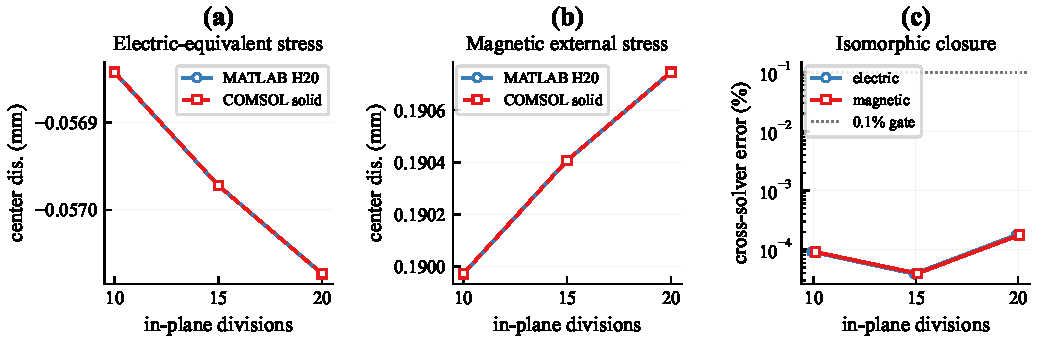
\includegraphics[width=0.98\textwidth]{Fig_03_isomorphic_solid_closure.pdf}
\caption{MATLAB H20 与 COMSOL 二次三维实体的同构闭合。前两幅图分别比较电、磁等效应力工况的中心位移，右图给出中心点相对差；自由端中点的完整数值见表~\ref{tab:iso_free_mid}。}
\end{figure}

\section{全半径曲壳 20/30 网格结果}

\subsection{网格收敛}

四个半径均完成 U/X 两种分布和三类载荷的 20$\times$20、30$\times$30 复算，共 48 条原始结果；最终 30$\times$30 主结果为 24 条。输入护照显示 U、X 各自跨网格材料数值哈希唯一，节点实际半径与声明半径一致。

\begin{table}[H]
\centering
\caption{各半径六类中心位移的 20$\rightarrow$30 网格变化}
\label{tab:radius_mesh_summary}
\begin{tabular}{rrrrl}
\toprule
$R$/m & 曲率/$\mathrm{m}^{-1}$ & 最大变化/\% & 平均变化/\% & 0.5\% 门槛 \\
\midrule
\RadiusSummaryRows
\bottomrule
\end{tabular}
\end{table}

全部 24 个工况均通过 0.5\% 门槛；全表最大变化为 $0.00787753\%$，位于 $R=1.0$ m、U 分布的压力工况。30$\times$30 结果可以作为当前曲率参数比较的统一离散基准。

\subsection{24 个工况的逐项收敛结果}

按半径汇总的最大值能够快速判断门槛，但无法说明某一载荷是否系统地更敏感。表~\ref{tab:full_20_30_results}因此保留全部 24 个正式工况。压力工况的 20$\rightarrow$30 变化为 0.003535\%--0.007878\%，平均为 0.005350\%；电致与磁致工况均为 0.000714\%--0.003216\%，平均为 0.001833\%。全表平均变化为 0.003006\%，中位数为 0.002241\%，远低于 0.5\% 门槛。

{\small
\begin{longtable}{llrrrr}
\caption{四半径、两分布、三载荷的完整 20/30 网格复算}\label{tab:full_20_30_results}\\
\toprule
载荷 & $R$/m--分布 & $w_{20}$/mm & $w_{30}$/mm & 变化/\% & $|w_R|/|w_{\infty}|$ \\
\midrule
\endfirsthead
\multicolumn{6}{c}{表~\thetable\ （续）}\\
\toprule
载荷 & $R$/m--分布 & $w_{20}$/mm & $w_{30}$/mm & 变化/\% & $|w_R|/|w_{\infty}|$ \\
\midrule
\endhead
\midrule
\multicolumn{6}{r}{续下页}\\
\endfoot
\bottomrule
\endlastfoot
压力 & 1.0--U & $-2.06951495$ & $-2.06935194$ & 0.007878 & 0.972659 \\
压力 & 1.0--X & $-1.75916901$ & $-1.75905248$ & 0.006624 & 0.971660 \\
压力 & 0.4--U & $-1.96027889$ & $-1.96016405$ & 0.005859 & 0.921338 \\
压力 & 0.4--X & $-1.66717212$ & $-1.66709368$ & 0.004705 & 0.920864 \\
压力 & 0.3--U & $-1.88198075$ & $-1.88188008$ & 0.005349 & 0.884542 \\
压力 & 0.3--X & $-1.60074839$ & $-1.60068092$ & 0.004215 & 0.884179 \\
压力 & 0.2--U & $-1.68110461$ & $-1.68102664$ & 0.004638 & 0.790134 \\
压力 & 0.2--X & $-1.42999398$ & $-1.42994343$ & 0.003535 & 0.789868 \\
\midrule
电致 & 1.0--U & $-0.05942182$ & $-0.05942373$ & 0.003216 & 1.137142 \\
电致 & 1.0--X & $-0.04885772$ & $-0.04885880$ & 0.002209 & 1.152563 \\
电致 & 0.4--U & $-0.06295361$ & $-0.06295316$ & 0.000714 & 1.204682 \\
电致 & 0.4--X & $-0.05170240$ & $-0.05170161$ & 0.001529 & 1.219624 \\
电致 & 0.3--U & $-0.06291040$ & $-0.06290962$ & 0.001234 & 1.203848 \\
电致 & 0.3--X & $-0.05163949$ & $-0.05163844$ & 0.002022 & 1.218133 \\
电致 & 0.2--U & $-0.06171538$ & $-0.06171448$ & 0.001470 & 1.180978 \\
电致 & 0.2--X & $-0.05063969$ & $-0.05063854$ & 0.002273 & 1.194546 \\
\midrule
磁致 & 1.0--U & $0.19852238$ & $0.19852877$ & 0.003216 & 1.137142 \\
磁致 & 1.0--X & $0.35151755$ & $0.35152531$ & 0.002209 & 1.152563 \\
磁致 & 0.4--U & $0.21032173$ & $0.21032023$ & 0.000714 & 1.204682 \\
磁致 & 0.4--X & $0.37198423$ & $0.37197854$ & 0.001529 & 1.219624 \\
磁致 & 0.3--U & $0.21017738$ & $0.21017479$ & 0.001234 & 1.203848 \\
磁致 & 0.3--X & $0.37153156$ & $0.37152405$ & 0.002022 & 1.218133 \\
磁致 & 0.2--U & $0.20618494$ & $0.20618191$ & 0.001470 & 1.180978 \\
磁致 & 0.2--X & $0.36433832$ & $0.36433004$ & 0.002273 & 1.194546 \\
\end{longtable}
}

电致与磁致的网格变化在每一个半径和分布上几乎逐项相等，这不是两组独立随机误差恰好相同，而是当前线性模型中两类外场载荷在空间上形成比例载荷向量。压力载荷的变化略大，但最大值仍只有门槛的 1.58\%。U 分布的全表平均变化为 0.003083\%，X 分布为 0.002929\%，二者没有显示出某一分布在数值上明显更难收敛。

从判定角度看，曲率扫描中任何 1\% 量级的趋势都不可能由表中的 20/30 网格差单独解释；即使最小的机械交互量只有约 0.027 个百分点，也仍需要与三倍离散界单独比较，而不能只引用“全部网格通过”这一总体结论。后文因此同时报告响应幅值、归一化比值和交互/网格界之比。

\subsection{\texorpdfstring{30$\times$30 正向响应}{30x30 正向响应}}

用于曲率归一化的平板参考值为：U 分布下压力、电致、磁致中心位移分别为 $-2.12751986$、$-0.05225709$、$0.17458575$ mm；X 分布下分别为 $-1.81035762$、$-0.04239145$、$0.30499453$ mm。

\begin{table}[H]
\centering
\caption{四个有限半径的 30$\times$30 中心位移}
\label{tab:curved_30_results}
\small
\begin{tabular}{rrr@{\hspace{1.0em}}rrr}
\toprule
$R$/m & 分布 & 压力/mm & 300 V/mm & 200 A/mm & 最大网格变化/\% \\
\midrule
1.0 & U & $-2.06935194$ & $-0.05942373$ & $0.19852877$ & 0.0079 \\
1.0 & X & $-1.75905248$ & $-0.04885880$ & $0.35152531$ & 0.0066 \\
0.4 & U & $-1.96016405$ & $-0.06295316$ & $0.21032023$ & 0.0059 \\
0.4 & X & $-1.66709368$ & $-0.05170161$ & $0.37197854$ & 0.0047 \\
0.3 & U & $-1.88188008$ & $-0.06290962$ & $0.21017479$ & 0.0053 \\
0.3 & X & $-1.60068092$ & $-0.05163844$ & $0.37152405$ & 0.0042 \\
0.2 & U & $-1.68102664$ & $-0.06171448$ & $0.20618191$ & 0.0046 \\
0.2 & X & $-1.42994343$ & $-0.05063854$ & $0.36433004$ & 0.0035 \\
\bottomrule
\end{tabular}
\end{table}

压力位移绝对值随曲率增大而单调降低：从 $R=1.0$ m 到 $R=0.2$ m，U 和 X 分布分别降低 18.77\% 和 18.71\%。电致与磁致响应则在 $R=0.4$ m 附近达到本组离散半径中的最大值；两类载荷的归一化曲线一致，符合线性结构方程中载荷幅值缩放的预期。

\subsection{压力响应：曲率刚化与分布稳定性}

相对各自平板基线，$R=1.0$ m 时 U/X 压力位移已经分别下降 2.734\% 和 2.834\%；半径继续减小到 0.4、0.3 和 0.2 m 时，归一化位移依次约为 0.921、0.884 和 0.790。该结果表明，在当前 CFFF 边界和小变形 LRT5 模型内，曲率增加伴随横向压力柔度持续降低。这里用“伴随”而不直接宣称普遍因果，是因为本研究没有改变边界、厚度和弧长来分离全部几何机制。

U 与 X 的压力位移绝对值差约为 15\%，但二者相对各自平板基线的曲率曲线几乎重合。从 $R=1.0$ m 到 0.2 m，$|w_X|/|w_U|$ 仅由 0.85005 变为 0.85064。换言之，材料平均组分和厚度分布显著改变了压力响应的基线幅值，而曲率对两条归一化压力曲线的调制非常接近。这也是机械交互量仅为 $-0.0999$ 至 $-0.0266$ 个百分点的直接来源。

\subsection{电致与磁致响应：离散半径内的非单调峰值}

电致和磁致位移从平板到 $R=1.0$ m 增大，在 $R=0.4$ m 达到本组采样点中的最大值，随后在 $R=0.3$ m 基本保持，并在 $R=0.2$ m 回落。以电致为例，U 分布在 $R=0.4$ m 时比自身平板基线高 20.468\%，X 分布高 21.962\%；$R=0.3$ m 相对 $R=0.4$ m 仅低 0.069\% 和 0.122\%。这些差值高于相应的 20/30 网格变化，但半径采样仍然离散，因此正文只能表述为“$R=0.4$ m 是当前四个半径中的离散最大值”，不能进一步声称连续最优半径已经被精确定位。

电致与磁致的归一化结果在所有半径上相等到数值精度。磁/电位移绝对值之比为
\[
\frac{|w_M|}{|w_E|}=3.3409\quad(U),
\qquad
\frac{|w_M|}{|w_E|}=7.1947\quad(X),
\]
并且各自在四个半径上保持不变。

这说明在当前线性静力模型中，电场和磁场形成了不同幅值但空间比例固定的等效载荷。因而，电致与磁致曲线相同是线性装配结构的必然结果之一，不应被当作两份完全独立的曲率证据。

\subsection{U/X 原始幅值差异}

表~\ref{tab:x_u_effect}给出 X 相对 U 的原始位移变化。压力和电致位移在 X 分布下分别降低约 15\% 和 18\%，磁致位移则提高约 77\%。方向差异与两种材料组分对弹性、压电和压磁参数的不同贡献有关，但由于 X 分布的平均 BaTiO$_3$ 体积分数为 0.3、U 分布为 0.6，表中百分比不能解释为“仅改变梯度而总材料量不变”的纯梯度增益。更稳妥的术语是\textbf{U/X 分布效应}。

\begin{table}[H]
\centering
\caption{30$\times$30 结果中 X 分布相对 U 分布的位移变化}
\label{tab:x_u_effect}
\begin{tabular}{rrrr}
\toprule
$R$/m & 压力变化/\% & 电致变化/\% & 磁致变化/\% \\
\midrule
1.0 & $-14.995$ & $-17.779$ & $+77.065$ \\
0.4 & $-14.951$ & $-17.873$ & $+76.863$ \\
0.3 & $-14.942$ & $-17.916$ & $+76.769$ \\
0.2 & $-14.936$ & $-17.947$ & $+76.703$ \\
\bottomrule
\end{tabular}
\end{table}

三个载荷的 X/U 百分比随半径只发生缓慢变化：压力差缩小约 0.059 个百分点，电致降幅增加约 0.168 个百分点，磁致增幅降低约 0.362 个百分点。这一结果说明原始幅值主要由材料基线决定，曲率--分布耦合是在较大的基线差上叠加的百分点级效应。采用各自平板归一化后再计算 $I_R$，可以更清楚地区分这两部分。

\subsection{曲率--U/X 分布交互}

\begin{table}[H]
\centering
\caption{30$\times$30 曲率--U/X 分布交互及离散边界}
\label{tab:interaction}
\scriptsize
\begin{tabular}{rllrrr}
\toprule
$R$/m & 载荷 & $I_R$/百分点 & 最大网格变化/\% & $|I_R|$/网格界 & 判定 \\
\midrule
\InteractionRows
\bottomrule
\end{tabular}
\end{table}

12 个交互量全部高于三倍离散界。机械交互为 $-0.0999$ 至 $-0.0266$ 个百分点，表明曲率下 U/X 的归一化机械响应十分接近；电致和磁致交互为 $1.3568$ 至 $1.5421$ 个百分点，且同半径两者最大差仅 $1.602\times10^{-8}$ 个百分点。由此可将“曲率改变 U/X 分布对内禀致动的相对效果”作为当前可分辨的数值规律，其中本组最强交互位于 $R=1.0$ m。

\subsection{交互量的强度、方向与可分辨性}

机械交互为负，表示曲率相对平板基线对 X 分布压力响应的抑制略强于 U 分布；电致和磁致交互为正，表示曲率对 X 分布内禀致动的相对放大略强。机械交互的绝对值随曲率从 1.0 增至 5.0 m$^{-1}$ 而由 0.0999 降至 0.0266 个百分点；电/磁交互也由 1.5421 降至 1.3568 个百分点。因而，交互最强点并不与电致、磁致绝对位移的离散最大值重合：前者出现在 $R=1.0$ m，后者出现在 $R=0.4$ m。这个区别说明“响应最大”和“U/X 相对分离最大”是两个不同问题。

以交互绝对值除以同工况最大网格变化，机械工况的比值为 5.75--12.68，电致和磁致为 479.6--977.1。本文的正式判据要求该比值超过 3，因此 12 个点全部被分辨。即使机械交互数值很小，其最不利比值仍为 5.75；电/磁交互则远高于离散界。这里的“已分辨”只表示交互高于当前 20/30 网格噪声，不代表它已经通过实物测量，也不表示线性混合规则之外的材料不确定性已被计入。

曲率--分布交互的数值意义可以分两层理解。第一层是稳健的计算事实：在各自平板归一化后，U/X 曲线仍有可重复的分离。第二层是受模型约束的解释：这种分离可能来自曲率改变弯曲应变在厚度方向的权重，使不同层的弹性和耦合参数贡献发生变化。后者属于与方程结构一致的机制解释，而不是由当前数据唯一识别出的材料因果机制，正文应保留这一限定。

\begin{figure}[H]
\centering
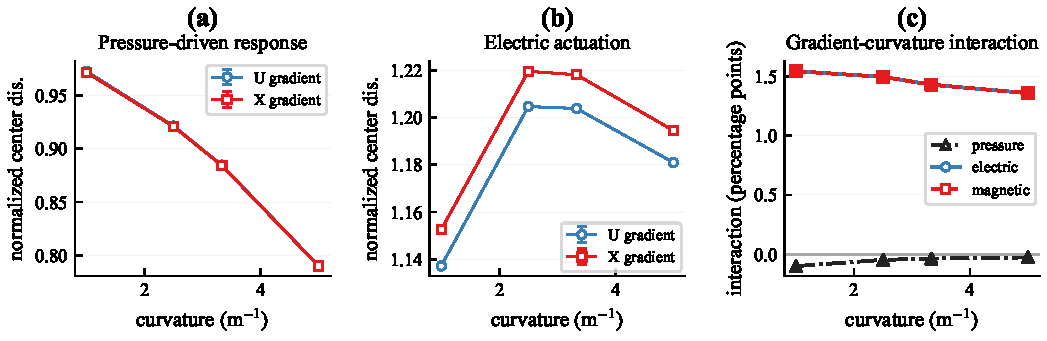
\includegraphics[width=0.98\textwidth]{Fig_04_all_radius_curvature_validation.pdf}
\caption{四个半径的 30$\times$30 响应及曲率--U/X 分布交互。位移误差棒采用对应的 20$\rightarrow$30 变化，交互图实心点表示超过三倍离散界。}
\end{figure}

\section{代表曲壳独立 COMSOL 结果}

\subsection{独立三维模型与径向探针}

代表工况取 U 分布、$R=0.4$ m、15 kPa 压力。COMSOL 模型为轴向 300 mm、弧长 300 mm、厚度 6 mm 的三维圆柱扇段，固支端为 $\theta=0$ 整个端面，外曲面受压；网格沿轴向和周向分别取 10/15/20，厚度固定 10 层。中心输出采用中面径向投影
\[
u_r=-v\sin\theta+w\cos\theta.
\]

使用径向投影而不是直接读取全局 $w$ 分量，是因为圆柱扇段不同周向位置的局部法向随 $\theta$ 旋转。若直接比较全局分量，几何坐标变换会被混入模型差异。当前中心探针位于轴向和弧向中点，COMSOL 输出先投影到该点的局部径向，再与 MATLAB LRT5 的法向位移比较。该处理统一了输出物理含义，但没有统一两种模型的运动学自由度，因此证据等级仍为 B 级。

\subsection{三维曲壳自身的网格演化}

\begin{table}[H]
\centering
\caption{$R=0.4$ m 代表曲壳的独立 COMSOL 网格结果}
\label{tab:curved_comsol_mesh}
\begin{tabular}{lrrrr}
\toprule
模型 & 面内网格 & 厚度网格 & 中心径向位移/mm & 相邻网格变化/\% \\
\midrule
COMSOL 三维实体 & 10$\times$10 & 10 & $-1.98666673$ & -- \\
COMSOL 三维实体 & 15$\times$15 & 10 & $-2.09847443$ & 5.6279 \\
COMSOL 三维实体 & 20$\times$20 & 10 & $-2.11872753$ & 0.9651 \\
MATLAB LRT5 & 20$\times$20 & 10 层 & $-1.96027889$ & -- \\
\bottomrule
\end{tabular}
\end{table}

COMSOL 的 15$\rightarrow$20 变化为 0.9651\%，通过 1\% 曲壳独立模型门槛。20$\times$20 时两种模型的位移符号和数量级一致，相对差为 8.0830\%。由于 MATLAB 使用 LRT5 曲壳、COMSOL 使用二次三维实体，这一差异用于量化模型形式敏感性，不作为跨软件数值误差。它与上一节的 A 级同构误差共同说明：当前软件实现能够在同构条件下闭合，而板壳降维与三维实体之间仍存在约 8\% 的模型层级差异。

从 10$\times$10 到 15$\times$15，COMSOL 中心径向位移增加 0.111808 mm，变化为 5.6279\%；从 15$\times$15 到 20$\times$20，增量缩小为 0.020253 mm，变化为 0.9651\%。后一增量只有前一增量的约 18.1\%，解随网格细化呈单调稳定趋势。由于只有三档网格且细化比不相同，本文不据此进行高阶 Richardson 外推，也不把 20$\times$20 称为严格的连续极限；“通过 1\% 门槛”是对当前代表模型离散稳定性的有限陈述。

\subsection{8.083\% 差异的尺度分解}

20$\times$20 时，COMSOL 三维实体与 MATLAB LRT5 的绝对差为 0.158449 mm，而 COMSOL 最近一次 15$\rightarrow$20 网格增量为 0.020253 mm，前者约为后者的 7.82 倍。由此可见，8.083\% 的总差异不太可能仅由 COMSOL 最后一档网格变化解释。与此同时，MATLAB 同半径压力工况的 20$\rightarrow$30 变化只有 0.005859\%，也远小于 8.083\%。因此，把主要剩余差异归入模型形式敏感性，比称作软件计算误差更符合现有证据。

可能贡献于该模型形式差异的因素包括：LRT5 将厚度方向位移场限制为一阶形式，而三维实体允许更完整的厚度翘曲；两种模型对横向剪切与曲率几何的表达不同；压力施加于三维外曲面，而板壳模型采用降维后的等效载荷；中心点法向位移虽已统一，但邻域内应力和应变场不要求一致。这些是基于模型结构的合理来源列表，当前一个代表工况无法定量拆分各项占比。

该代表模型的价值不在于证明 LRT5 与三维实体必须相差 8\%，而在于给正文提供一个独立的模型层级敏感性样本。它确认了符号、毫米量级和随网格细化的趋势，同时显示板壳降维在中等曲率下可能带来显著于数值离散误差的响应差异。因而，小论文可把 8.083\% 作为模型讨论项，但不能把它推广到其他半径、X 分布或电磁载荷。

\begin{figure}[H]
\centering
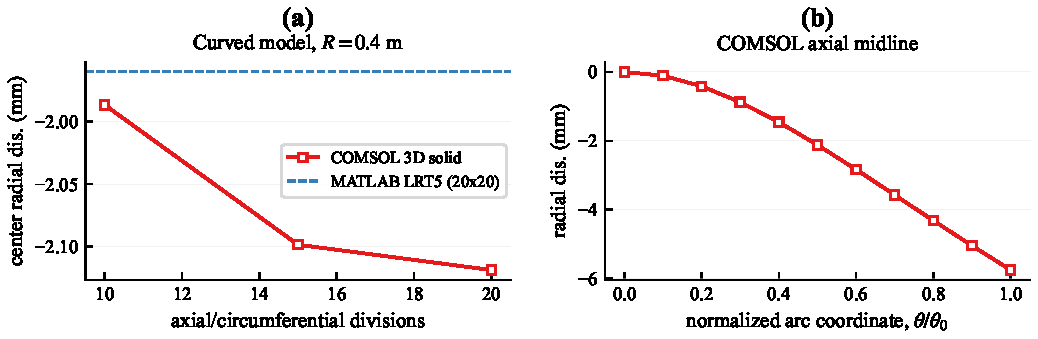
\includegraphics[width=0.95\textwidth]{Fig_05_curved_comsol_validation.pdf}
\caption{代表曲壳独立 COMSOL 结果。左图为网格收敛及 MATLAB LRT5 参考线，右图为 20$\times$20$\times$10 模型的轴向中线径向位移。}
\end{figure}

\section{位移反问题：加载反算与感生势审计}

\subsection{先区分两个不同的反问题}

“达到规定中心位移需要施加多大电势或磁标势”和“结构发生规定变形后，在开路边界下产生多大感生势”不是同一个问题。前者以外加载势为未知量，利用正向致动关系反算；后者以感生电势、磁标势为未知量，必须给定机械状态、电极开路条件、磁边界和参考势。原报告把两类量都称作“位移反推电势/磁势”，使 $78.4803$ V 和 $0.0309000$ A 被误读为产生 0.5 mm 位移所需的加载值。以下分别核对。

\subsection{目标位移所需外加载势、自洽回代与交叉施加}

当前平板正向基准给出：MATLAB 在 300 V 电势下的中心位移绝对值为 0.05225709493 mm，在 200 A 磁标势下为 0.1745857472 mm；COMSOL 20$\times$20$\times$10 直接场模型对应为 0.05788658849 mm 和 0.1907662164 mm。因此
\[
\begin{aligned}
|S_\phi^{\mathrm M}|&=1.741903164\times10^{-4}\ {\rm mm/V},&
|S_\phi^{\mathrm C}|&=1.929552950\times10^{-4}\ {\rm mm/V},\\
|S_\psi^{\mathrm M}|&=8.729287359\times10^{-4}\ {\rm mm/A},&
|S_\psi^{\mathrm C}|&=9.538310819\times10^{-4}\ {\rm mm/A}.
\end{aligned}
\]
按 $|\Phi_{\rm req}|=|w^*|/|S_\phi|$、$|\Psi_{\rm req}|=|w^*|/|S_\psi|$ 得到表~\ref{tab:inverse_actuation_loads}。A 是磁标势差的单位，不是电流。

\begin{table}[H]
\centering
\caption{达到目标中心位移所需的外加载势}
\label{tab:inverse_actuation_loads}
\scriptsize
\begin{tabular}{rrrrrrr}
\toprule
$|w^*|$/mm & MATLAB/V & COMSOL/V & 差/\% & MATLAB/A & COMSOL/A & 差/\% \\
\midrule
0.5 & 2870.4236 & 2591.2738 & $-9.7250$ & 572.7844 & 524.2018 & $-8.4818$ \\
1.0 & 5740.8473 & 5182.5476 & $-9.7250$ & 1145.5689 & 1048.4037 & $-8.4818$ \\
2.0 & 11481.6945 & 10365.0952 & $-9.7250$ & 2291.1378 & 2096.8073 & $-8.4818$ \\
\bottomrule
\end{tabular}
\end{table}

上述 COMSOL 数值不是把 MATLAB 结果换单位得到的。电致链在两个外侧活动层直接建立 Electrostatics 与 Piezoelectric Effect，磁致链在外侧活动层求解磁标势弱式场，再由 $H_3=-\partial\psi/\partial z$ 和 $q_{31},q_{32}$ 形成体内本构应力；两者均未施加预先计算的等效表面压力。先对表中每个 COMSOL 自身反算载荷建立目标专属工况并重新求解，所得结果列于表~\ref{tab:inverse_actuation_return}。这一步检验 COMSOL 链自身是否闭合，不直接检验 MATLAB 载荷。

\begin{table}[H]
\centering
\caption{COMSOL 自身灵敏度反算载荷的目标专属自洽回代}
\label{tab:inverse_actuation_return}
\scriptsize
\begin{tabular}{rrrrr}
\toprule
目标/mm & 电致回代/mm & 电致残差/\% & 磁致回代/mm & 磁致残差/\% \\
\midrule
0.5 & 0.500000232 & $4.6400\times10^{-5}$ & 0.500000000 & $3.9190\times10^{-10}$ \\
1.0 & 1.000003750 & $3.7504\times10^{-4}$ & 1.000000000 & $7.0907\times10^{-9}$ \\
2.0 & 1.999998220 & $8.8987\times10^{-5}$ & 2.000000000 & $1.2315\times10^{-8}$ \\
\bottomrule
\end{tabular}
\end{table}

若要真正检验 MATLAB 载荷跨到另一个模型后会发生什么，必须把 MATLAB 数值不作重标定地输入 COMSOL。表~\ref{tab:inverse_actuation_crossapply} 给出已经实际运行的 0.5 mm 交叉工况。

\begin{table}[H]
\centering
\caption{MATLAB 反算载荷原样施加到 COMSOL（0.5 mm 目标）}
\label{tab:inverse_actuation_crossapply}
\scriptsize
\begin{tabular}{lrrrr}
\toprule
通道 & MATLAB 反算载荷 & COMSOL 位移/mm & $|w_{\rm C}|/|w^*|$ & 相对目标差/\% \\
\midrule
电致 & 2870.4236 V & 0.553862904 & 1.107725808 & $+10.7726$ \\
磁致 & 572.7844 A & 0.546339605 & 1.092679211 & $+9.2679$ \\
\bottomrule
\end{tabular}
\end{table}

因此，表~\ref{tab:inverse_actuation_return} 只能证明“COMSOL 用自身灵敏度反算、再代回自身正向模型”能够闭合；表~\ref{tab:inverse_actuation_crossapply} 才是 MATLAB 载荷对 COMSOL 的直接交叉检验。MATLAB 使用 LRT5 板壳；电致 COMSOL 使用三维压电实体；磁致 COMSOL 使用三维实体、弱式磁标势场与单向应力耦合。9.27\%--10.77\% 的交叉位移差与两套灵敏度所给 8\%--10\% 的加载差相互一致，应报告为非同构模型形式敏感性，不能归为求解器计算错误，也不能声称任一方已证明另一方的绝对正确性。

\subsection{与 Zhang 等（钱沈云为合著者）已发表结果的比较}

仓库中未发现钱沈云学位论文原文；当前可核对的正式资料是 Zhang 等 2026 年发表的热--磁--电--弹板论文，钱沈云为合著者。其已发表基准是 $300\ {\rm mm}\times300\ {\rm mm}\times6\ {\rm mm}$ CFFF 方板，不是四半径圆柱壳。论文给出 300 V 电致中心位移 $-0.0523$ mm，200 A 磁致中心位移为现模型 0.175 mm、COMSOL 0.173 mm；论文 COMSOL 还采用势载荷换算等效应力的方法，而不是独立反向传感 PDE。本文对照其 Eqs.~(1)--(4)、(9)--(10)、(51)--(54) 以及 Tables~1--5 的本构、离散和正向结果，而不把作者身份当作数值正确性的替代证据。

用论文正向位移表反算 0.5 mm 外加载势，现模型得到 2868.0688 V 和 571.4286 A，论文 COMSOL 得到 2868.0688 V 和 578.0347 A。本项目 MATLAB 的 2870.4236 V、572.7844 A 相对论文现模型分别高 0.0821\% 和 0.2373\%。所以加载反算与已发表正向结果相容；但论文没有发表位移反推感生电势/磁势的 COMSOL 表，不能据此证明后文 $78.4803$ V、$0.0309000$ A 的感生势正确。

\subsection{感生势的局部本构、量纲与条件性}

原程序在“无外加热源”条件下并没有强制 $\Delta T=0$。MATLAB 离散系统先由
\[
\mathbf K_{Tu}\mathbf Q_d+\mathbf K_{TT}\Delta\mathbf T_s=\mathbf0
\]
求得热--机互易温度响应 $\Delta\mathbf T_s$；随后它以
$-\mathbf K_{\phi u}\mathbf Q_d-\mathbf K_{\phi T}\Delta\mathbf T_s$ 和
$-\mathbf K_{\psi u}\mathbf Q_d-\mathbf K_{\psi T}\Delta\mathbf T_s$ 作为势方程右端。故“无外加热源”与“强制等温 $\Delta\mathbf T_s=\mathbf0$”是两个不同工况。

为了审查局部量纲和可逆性，取某层代表温度量 $\Delta T_s$，令
\[
s=\varepsilon_{xx}+\varepsilon_{yy},\qquad
a=e\,s+p\Delta T_s,\qquad b=q\,s+\tau\Delta T_s.
\]
再额外采用局部一维诊断条件 $D_3=B_3=0$，才有
\[
\begin{bmatrix}g_{\rm eff}&k\\k&r\end{bmatrix}
\begin{bmatrix}E_3\\H_3\end{bmatrix}
=-\begin{bmatrix}a\\b\end{bmatrix}.
\]
显式求逆得到
\[
E_3=-\frac{ra-kb}{g_{\rm eff}r-k^2},\qquad
H_3=\frac{ka-g_{\rm eff}b}{g_{\rm eff}r-k^2},
\]
单层势差为
\[
\Delta\phi=-E_3h_\ell,\qquad \Delta\psi=-H_3h_\ell.
\]
这里 $e$ 的单位为 $\mathrm{C/m^2}$，$q$ 为 $\mathrm{N/(A\,m)}=\mathrm T$，$g_{\rm eff}$ 为 $\mathrm{F/m}$，$k$ 为 $\mathrm{s/m}$，$r$ 为 $\mathrm{H/m}$，$p$ 为 $\mathrm{C/(m^2\,K)}$，$\tau$ 为 $\mathrm{T/K}$；$E_3$、$H_3$、$\Delta\phi$、$\Delta\psi$ 的单位依次为 V/m、A/m、V、A。当前参数给出
\[
e_{31}=-9.8715904271\ {\rm C/m^2},\qquad
g_{\rm eff}=8.1360785066\times10^{-9}\ {\rm F/m},
\]
\[
k=1.755\times10^{-8}\ {\rm s/m},\qquad
r=7.536\times10^{-5}\ {\rm H/m},\qquad
g_{\rm eff}r-k^2=6.1282687376\times10^{-13}\ {\rm s^2/m^2}>0.
\]
直接对带单位矩阵计算条件数会混入 V/m 与 A/m 的尺度差。采用
\[
\mathbf W=\operatorname{diag}(g_{\rm eff}^{-1/2},r^{-1/2}),\qquad
\mathbf W
\begin{bmatrix}g_{\rm eff}&k\\k&r\end{bmatrix}
\mathbf W=
\begin{bmatrix}1&\rho\\\rho&1\end{bmatrix},
\]
\[
\rho=\frac{k}{\sqrt{g_{\rm eff}r}}=0.02241295,\qquad
\kappa_2=\frac{1+|\rho|}{1-|\rho|}=1.04585
\]
后可见，局部 $2\times2$ 本构反演在单位归一化后条件良好。这里的逐点 $D_3=B_3=0$ 比真实浮置电极的面积积分零净自由电荷条件更强，磁场也不存在无需说明空气域和开放边界的通用“开路”条件。因此它只能是局部本构诊断。尚未保存的是全局有限元感生势矩阵的尺度化条件数与相对残差，也尚未在 COMSOL 中建立空气域、磁势规范和完整 $\phi/\psi/T$ 自由度，不能把局部稳定外推为全局传感 PDE 已验证。

\subsection{原感生势表的真实含义}

原 MATLAB 数值不是 0.5/1/2 mm 三次独立求解，而是同一个 30$\times$30 基准结果按目标位移缩放。修正后基准中心位移为 2.1275198619 mm，十层“层平均势自由度”的极差为 333.9366869825 V 和 0.1314808939 A，随后统一乘以 $|w^*|/2.1275198619$。COMSOL 一侧也只运行一次 15 kPa 三维力学模型，得到中心位移 2.269513209 mm；再读取各层 $\varepsilon_{xx},\varepsilon_{yy}$，套用与 MATLAB 相同的局部代数本构，并乘以目标位移缩放系数。模型中没有独立电势、磁标势或温度自由度。

\begin{table}[H]
\centering
\caption{探索性的层均感生势跨度：20$\times$20 三维力学、每物理层 5 个厚度单元；无外加热源且保留互易温度响应}
\label{tab:inverse_sensing_exploratory}
\scriptsize
\begin{tabular}{rrrrrr}
\toprule
$|w^*|$/mm & MATLAB 30$\times$30/V & 三维力学后处理/V & MATLAB 30$\times$30/A & 三维力学后处理/A & 共享差/\% \\
\midrule
0.5 & 78.4803 & 81.1999 & 0.0309000 & 0.0319709 & 3.4654 \\
1.0 & 156.9605 & 162.3999 & 0.0618001 & 0.0639417 & 3.4654 \\
2.0 & 313.9211 & 324.7998 & 0.1236002 & 0.1278834 & 3.4654 \\
\bottomrule
\end{tabular}
\end{table}

三个位移点的严格比例是缩放算法直接规定的，不是独立幅值求解发现的线性；电势与磁势的 3.4654\% 完全相同，是因为二者依赖同一个机械应变比例，不是两个统计独立的验证样本。输出定义又是十层层平均势自由度的最大值减最小值，并非中心点势、端子电压或外加载势。因此本表只能保留为探索性本构后处理，不进入“已由 COMSOL 证明正确”的结果集合。

温度边界会显著改变该探索性结果。表~\ref{tab:inverse_sensing_thermal_boundary} 在同一 0.5 mm、20$\times$20 三维力学、每物理层 5 个厚度单元条件下，比较强制 $\Delta T_s=0$ 与无外加热源但由互易热方程求得 $\Delta T_s$ 的结果。

\begin{table}[H]
\centering
\caption{0.5 mm 感生势后处理对温度边界的敏感性}
\label{tab:inverse_sensing_thermal_boundary}
\scriptsize
\begin{tabular}{lrrrr}
\toprule
温度处理 & MATLAB/V & 三维力学后处理/V & MATLAB/A & 三维力学后处理/A \\
\midrule
强制等温 $\Delta T_s=0$ & 68.906264 & 71.294157 & 0.053265891 & 0.055111779 \\
无外加热源，保留互易响应 & 78.480275 & 81.199948 & 0.030900039 & 0.031970856 \\
\bottomrule
\end{tabular}
\end{table}

因此 $78.4803$ V 和 $0.0309000$ A 不能再标为“等温结果”。电通道相对强制等温增加约 13.9\%，磁通道则减少约 42.0\%；若不写清热边界，仅凭位移目标无法唯一确定这两个势跨度。

原九行“MATLAB 10/15/20 网格”表还重复使用了同一个 MATLAB 30$\times$30 参考值。一次新鲜的 MATLAB 10$\times$10 修正复跑为 78.431689 V 和 0.030880910 A，并非原表的 78.4803 V 和 0.0309000 A。故本次删除原九行表，避免把复制参考值误报为三档网格收敛。

\subsection{钱沈云相关旧程序为何给出更大感生势}

钱沈云相关程序同工况复跑在 2 mm 时得到 658.5854897351 V 和 0.6815705005 A，而当前修正值为 313.9210993579 V 和 0.1236001565 A。差异不能由相同平板几何、中心点定义或网格解释。代码审计显示，线性单元程序在处理每个物理层时，均把该层热释电系数 PE 与热释磁系数 PM 写入全部 10 个势自由度；十个物理层依次装配后，热释耦合系数恰为本构输入的 10 倍。旧值/修正值倍率不是共同的 10 倍，是因为机械项和温度项叠加方向不同，磁势通道还存在符号竞争。

这说明同源代码复跑到机器精度只证明“旧代码可以重现旧输出”，不能证明旧装配在数学上正确。也不能简单把最终势值除以 10；必须在修正热释耦合矩阵后重新求解。旧程序缺陷集中在 \texttt{SF\_ElemComptLIN851T5MEEP\_V4.m} 第 184--193、241--242、452--453 行附近的层自由度写入和全局装配。若正文声明强制 $\Delta T=0$，就不能同时引用含非零温度响应的 SensM\_T 数值；若采用“无外加热源”，方程必须显式包含 $\mathbf K_{\phi T}\Delta\mathbf T_s$ 与 $\mathbf K_{\psi T}\Delta\mathbf T_s$。

\subsection{用户所示圆柱壳表的可比性限制}

用户截图中的前人圆柱壳写为 $R=0.6$ m、圆心角 0.5 rad、曲边 600 mm、10 kPa、自由端中点输出；当前正式四半径模型则采用弧长 300 mm、$R=1.0,0.4,0.3,0.2$ m、15 kPa、几何中心法向位移，并比较 U/X 两种分布。几何、压力、测点和材料分布均不同，不能直接用截图中的 $-3.7431$ mm 判断当前表对错。

截图参数内部也需要回查：若 $R=0.6$ m、$\alpha=0.5$ rad，则 $b=R\alpha=0.3$ m，不是 0.6 m；若曲边确为 0.6 m，则圆心角应为 1 rad。仓库中的钱沈云相关代码虽包含未发表的圆柱壳输入资产，但 Zhang 等论文正文只发表平板，原圆柱壳脚本还使用 4800 V、1400 A 等不同载荷。因此本报告的四幅圆柱壳图只标为“本研究参数化几何与载荷示意”，不称为钱沈云论文算例。

\section{综合讨论}

\subsection{不同百分比不能放在同一误差概念下}

本文出现的百分比跨越约五个数量级，但它们并不是同一个“准确率”的不同表现。表~\ref{tab:error_scale_hierarchy}按比较对象重新排列这些数值。最小的 $0.0001769\%$ 是固定网格、同构运动学和同一探针下的跨求解器差；$0.0078775\%$ 是 MATLAB 曲壳 20/30 网格变化；$0.9651\%$ 是独立 COMSOL 三维曲壳自身的最近网格变化；3.4654\% 只是同一感生势本构后处理对不同机械场的共享尺度差；8.0830\% 是曲壳 LRT5 与三维实体差；8.4818\%--9.7250\% 是两种非同构正向模型的反算载荷差；9.2679\%--10.7726\% 是 MATLAB 载荷实际跨到 COMSOL 后的目标位移差。分母和问题不同，因此不能据此给软件排出单一优劣顺序。

\begin{table}[H]
\centering
\caption{当前最新结果中的数值差异层级及其含义}
\label{tab:error_scale_hierarchy}
\small
\begin{tabularx}{\textwidth}{>{\raggedright\arraybackslash}p{0.23\textwidth}>{\raggedright\arraybackslash}p{0.15\textwidth}YY}
\toprule
指标 & 当前数值 & 回答的问题 & 不应被解释为 \\
\midrule
H20--二次实体同构差 & 最大 0.0001769\% & 固定离散下两套机械核实现是否一致 & 连续解的网格误差 \\
MATLAB 曲壳 20/30 变化 & 最大 0.0078775\% & 四半径参数结果是否受当前网格主导 & MATLAB--COMSOL 软件差 \\
外部平板表格差 & 0.010\%--0.92\% & 当前平板是否落入已发表同工况量级 & 自由度级独立闭合 \\
COMSOL 曲壳 15/20 变化 & 0.9651\% & 独立三维曲壳最近一次细化是否稳定 & LRT5 理论误差 \\
感生势后处理共享差 & 3.4654\% & 两种机械应变场经同一局部本构后的尺度差 & 独立电、磁 PDE 的两个误差样本 \\
LRT5--三维实体差 & 8.0830\% & 降维运动学改变后的模型敏感性 & MATLAB 或 COMSOL 计算错误 \\
加载反算模型差 & 8.4818\%--9.7250\% & 两种非同构正向致动模型的所需载荷差 & 同构求解器误差 \\
MATLAB 载荷交叉施加差 & 9.2679\%--10.7726\% & MATLAB 0.5 mm 反算载荷输入 COMSOL 后的目标位移差 & 任一模型的绝对正确性证明 \\
\bottomrule
\end{tabularx}
\end{table}

这张表也直接回答“2\% 是否偏大”。若比较的是完全同构的平板机械核，当前证据表明 2\% 明显偏大，因为实际差只有 $10^{-4}\%$ 量级；出现 2\% 时应优先检查运动学、载荷面、材料换算、边界和探针。若比较的是 LRT5 与三维实体，或不同正向场模型反算的加载势，则百分数中包含模型形式，不能套用同构 0.1\% 门槛。对于感生势，因当前 COMSOL 没有独立 $\phi/\psi$ 自由度，3.4654\% 甚至不能称作求解器差。判断偏差是否合理的前提，是先确认比较属于表中的哪一行。

\subsection{从平板闭合到曲率规律的论证链}

当前证据链的第一步是外部平板基准。三类载荷相对公开表格均低于 1\%，说明单位、方向和总体量级没有明显错误。第二步是三维实体同构闭合：在排除板壳降维因素后，两个求解器的双探针差小于 1 nm，证明外应力机械核的实现可以达到远低于 0.1\% 的一致性。第三步才是 MATLAB LRT5 的四半径研究；所有 24 个正式工况完成 20/30 复算，使曲率趋势拥有显式离散边界。这个顺序避免了用一个未验证的曲壳模型直接讨论材料规律。

曲率结果内部又包含三层信息。原始位移说明不同 U/X 分布对三类载荷的幅值影响方向不同；各自平板归一化结果说明曲率对压力和内禀致动的调制形式不同；交互量进一步量化 U/X 归一化曲线的分离是否高于网格界。三层指标共同显示：压力响应随曲率单调减弱，电/磁响应在四个采样半径中于 $R=0.4$ m 最大，而 U/X 的相对分离在 $R=1.0$ m 最大。若只展示一张绝对位移图，这三个结论容易被混为一个“最佳半径”。

独立 COMSOL 曲壳把论证链延伸到不同运动学层级。其作用不是把 8.083\% 消除到零，而是显示在同构机械核已经闭合后，降维板壳与三维实体仍可能产生可见差异。这使曲率规律的表述更审慎：MATLAB LRT5 内部的相对趋势具有很小离散误差，但绝对位移向三维实体或真实结构外推时，应保留模型形式敏感性。

\subsection{U/X 分布效应的可发表表述}

U/X 原始比较中，X 分布的平均 BaTiO$_3$ 体积分数只有 U 的一半。因此，直接写成“功能梯度使磁致位移提高 77\%”会把平均材料组分变化与厚度重分布合并，并可能造成过强的因果表述。更准确的结果句是：“在本文定义的 U/X 两种材料分布下，X 分布相对 U 分布使压力和电致位移分别降低约 15\% 和 18\%，使磁致位移提高约 77\%。”这一句完整绑定了分布定义和参数范围。

归一化交互能够提供更接近曲率调制的结果。各模式分别用自身平板值归一化后，平均组分造成的大部分基线幅值差被抵消；剩余 1.3568--1.5421 个百分点的电/磁交互说明，曲率对 X 分布致动的相对放大略高于 U 分布。即便如此，归一化并不能数学上完全消除材料参数非线性或混合规则影响，因此正文宜称“曲率--U/X 分布交互”，而不是不加限定的“纯梯度--曲率耦合”。

表~\ref{tab:claim_language}把当前证据可支撑的论文语言与越界表述对应起来。该表不是质量控制记录，而是对数值结论含义的学术分析，可直接用于结果与讨论章节的措辞统一。

\begin{table}[H]
\centering
\caption{当前证据支持的结果表述边界}
\label{tab:claim_language}
\small
\begin{tabularx}{\textwidth}{YY}
\toprule
当前结果可支持 & 当前结果不能单独支持 \\
\midrule
同构三维机械核在六组载荷--网格组合中最大差为 0.0001769\% & MATLAB 与 COMSOL 对所有耦合 PDE 均天然无误差 \\
四个有限半径、两分布、三载荷的 30$\times$30 结果均通过 20/30 网格门槛 & $R=0.4$ m 是连续半径域中的全局最优值 \\
U/X 分布下原始响应与归一化曲率响应存在定量差异 & 保持平均材料组分不变时的纯梯度因果效应 \\
$R=0.4$ m 三维实体与 LRT5 相差 8.083\%，且差异大于最近网格增量 & 所有半径和所有载荷下模型形式差均固定为 8.083\% \\
MATLAB 与 COMSOL 的 0.5/1/2 mm 反算均分别完成自身模型回代；0.5 mm MATLAB 载荷交叉输入 COMSOL 后的目标差为 9.27\%--10.77\%，MATLAB 值与论文正向表反算差低于 0.24\% & 自身回代已独立证明另一模型，或由此证明真实器件性能 \\
原感生势表可作为层均势自由度极差的探索性后处理记录 & 原表已经得到独立 COMSOL 电势/磁标势 PDE 验证 \\
\bottomrule
\end{tabularx}
\end{table}

\subsection{数值实验与实物试验的边界}

本研究已经完成的 MATLAB/COMSOL 建模、参数控制、网格重复计算和交叉比较，均属于数值实验。称其为“实验”是准确的，因为输入变量、对照组和验收指标均被明确控制，结果也可以重复运行。它所检验的是方程实现、离散稳定性和模型趋势，而不是材料样件在仪器中的实际输出。

尚未完成的是实物试验：没有制备与模型相同的 BaTiO$_3$/CoFe$_2$O$_4$ 分层曲壳，也没有在 15 kPa、300 V、200 A 或规定 0.5 mm 位移下使用传感器采集数据。因此，“全部结果没有实验支撑”这一说法过于笼统，容易否定已经完成的数值实验；更准确的表述应为：“本文结论已有多层数值实验支撑，但尚无实物样件与台架测量支撑。”这一区分不影响数值方法章节成立，只限制真实器件性能的工程外推。

从小论文结构看，当前最完整的主体是“同构平板机械核验证--四半径 U/X 曲壳响应--交互量与网格界--代表三维曲壳敏感性”这一条链。加载反算可作为“各链自身回代 + MATLAB 载荷向 COMSOL 交叉施加”的扩展结果；感生势只能放入局限性或后续工作，并明确标注尚未独立求解电势/磁标势 PDE。这样的组织把已闭合的内容放在主结论，把尚未自由度同构的内容放在模型讨论中，不需要依赖未完成的实物数据来填补数值论证。

\section{综合结论与适用边界}

\begin{enumerate}[label=\arabic*.,leftmargin=2.3em]
\item 当前平板压力、电致和磁致位移相对已发表板模型与 COMSOL 表格的差异为 0.010\%--0.92\%，符号、测点和数量级均一致。这一外部基准说明平板正向模型没有百分数级系统偏移，但不替代独立同构验证。
\item MATLAB H20 与 COMSOL 二次三维实体的六组同构结果全部通过 0.1\% 门槛，中心点最大差为 $0.0001769\%$，双探针最大绝对差小于 1 nm。磁/电位移比还精确复现外应力幅值比，说明当前机械核在平衡、线性比例和跨软件点值上同时闭合。
\item 四个正文半径的 U/X、压力/电致/磁致共 24 个 30$\times$30 工况均有 20$\times$20 复算，最大网格变化仅 $0.00787753\%$，全表平均为 0.003006\%。曲率趋势和交互量已具有显式离散边界。
\item 压力响应随曲率增加单调减弱；电致和磁致响应在 $R=0.4$ m 取得四个采样半径中的最大值，但 $R=0.3$ m 与其非常接近，因此不能把 $R=0.4$ m 外推为连续域全局最优半径。
\item X 相对 U 使压力和电致位移分别降低约 15\% 和 18\%，使磁致位移提高约 77\%。由于两种分布的平均 BaTiO$_3$ 体积分数不同，这些值应称为 U/X 分布效应。各自平板归一化后的电致/磁致曲率--分布交互为 $1.3568$--$1.5421$ 个百分点，12 个交互点均高于三倍离散界。
\item 代表曲壳 COMSOL 自身达到 0.9651\% 的 15$\rightarrow$20 网格变化；与 LRT5 的 8.0830\% 差异是最近网格增量的约 7.82 倍，属于运动学和载荷降维共同影响下的模型形式敏感性，不能表述为求解器误差。
\item 位移反问题已拆成两条链。达到 0.5 mm 中心位移时，MATLAB/COMSOL 所需外加载势分别为 2870.4236/2591.2738 V 与 572.7844/524.2018 A；三组 COMSOL 载荷只证明 COMSOL 链自身闭合，而 MATLAB 的 0.5 mm 载荷原样输入 COMSOL 后得到 0.553863/0.546340 mm，目标差为 10.7726\%/9.2679\%。MATLAB 值与 Zhang 等已发表正向表反算值的差为 0.0821\% 和 0.2373\%。原 78.4803 V、0.0309000 A 是无外加热源但保留互易温度响应的一次机械解缩放后的层均感生势极差，不是外加载势；COMSOL 侧没有独立 $\phi/\psi/T$ PDE，故该表降级为探索性后处理。
\item 钱沈云相关程序的旧感生势可以同源复现，但代码审计发现热释电/热释磁矩阵对十层势自由度重复装配，装配系数恰为输入本构值的 10 倍。同源复跑会复现同一缺陷，不能作为旧值正确性的独立证据；修正必须在矩阵层完成，不能把最终输出简单除以 10。
\end{enumerate}

上述结论的适用范围限于当前几何、CFFF 边界、线性小变形假设、材料线性混合规则、10 层物理离散和静力载荷。H20 同构链只闭合外应力机械核；独立 COMSOL 曲壳目前只有 $R=0.4$ m、U 分布、压力载荷一个代表工况；加载反算依赖固定载荷形态下的线性正向灵敏度；感生势尚未形成完整独立传感 PDE。对其他边界、层数、材料参数、强场非线性或不同半径，本文不给出未经计算的定量外推。

本文 MATLAB/COMSOL 求解、网格复算、参数扫描与交叉对照均属于已经完成的数值实验，足以支撑算法一致性、离散收敛和当前参数域内的趋势结论。尚未开展的是实物样件和台架仪器测量，因此真实器件性能不能直接由本文数值替代。论文正文应据此清楚区分 A 级实现验证、B 级模型敏感性、数值参数规律与尚无实物试验支撑的工程外推。

\end{document}
